% Prof. Dr. Ausberto S. Castro Vera
% UENF - CCT - LCMAT - Curso de Ci\^{e}ncia da Computa\c{c}\~{a}o
% Campos, RJ,  2020
% Disciplina: Paradigmas de Linguagens de Programa\c{c}\~{a}o
% Aluno: Javier Ernesto


\chapterimage{img_superior}
\chapter{ Aplica\c{c}\~{o}es da Linguagem Kotlin}
A linguagem de programação Kotlin é usada por mais de 60\% dos desenvolvedores Android profissionais. Ela ajuda a aumentar a produtividade, a satisfação dos desenvolvedores e a segurança do código.

\section{Android}
O Kotlin é uma linguagem compatível com Android concisa,
expressiva e projetada para ser type- e null-safe (ter segurança de tipos e de nulos). Ele funciona perfeitamente com a linguagem Java, portanto, os desenvolvedores que gostam de Java podem continuar a utilizá-lo, ao mesmo tempo que adicionam código Kotlin e usam as bibliotecas dessa linguagem. Além disso, muitos desenvolvedores Android já descobriram que o Kotlin torna o desenvolvimento mais rápido e divertido, então queremos oferecer um suporte melhor a esses usuários do Kotlin

\subsection{Hello word}
Segue um exemplo de um codigo em Kotlin no Android
mostrando o hello word.
\begin{lstlisting}[label={lst:example1}, language=Kotlin]
  public class MainActivity extends AppCompatActivity {
 
    @Override
    protected void onCreate(Bundle savedInstanceState) {
        super.onCreate(savedInstanceState);
        setContentView(R.layout.activity_main);
        TextView textView = findViewById(R.id.textView);
        Button button = findViewById(R.id.button);
        button.setOnClickListener(new View.OnClickListener() {
            @Override
            public void onClick(View v) {
                textView.setText("Hello World with Kotlin is better");
            }
        });
    }
}
}   
\end{lstlisting}


O resultado no dispositivo moile será assim:

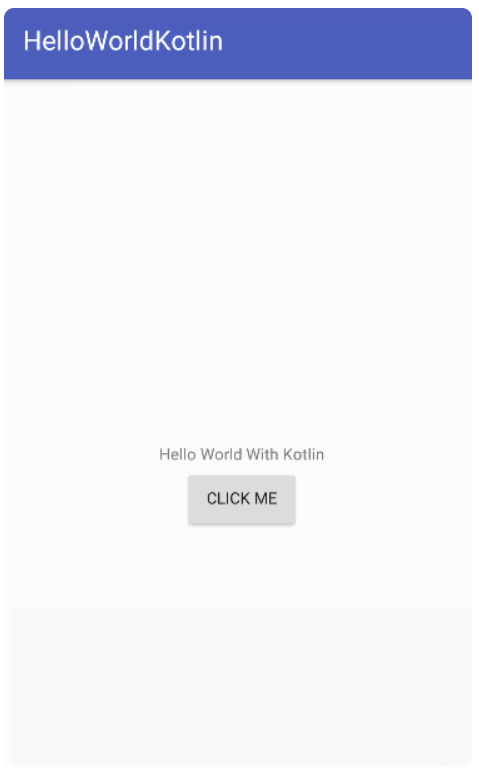
\includegraphics[ width=6cm, height=10cm]{HelloWordKotlin.PNG}


%%%--------------------------------------------------------------------
\section{O algoritmo Quicksort}
\begin{lstlisting}[label={lst:example1}, language=Kotlin]
      fun quicksort(items:List<Int>):List<Int>{
        if (items.count() < 2){
            return items
        }
        val pivot = items[items.count()/2]
        //pivot vai receber o valor central do vetor
        val equal = items.filter { it == pivot }
        //pegando o valor igual a do pivot
    
        val less = items.filter { it < pivot }
        //pegando o valor inferior ao pivot
    
        val greater = items.filter { it > pivot }
        //pegando o valor superior ao pivot

        return quicksort(less) + equal + quicksort(greater)
        //contatena os vetores e chama a funcao denovo
        }
    fun main(args: Array<String>) {
       println("Lista Original:")
        val numbers = listOf<Int>(2, 4, 7, 3, 6, 9, 5, 1, 0)
        println(numbers) //[2, 4, 7, 3, 6, 9, 5, 1, 0]
        println("Lista ordenada:")
        val ordered =  quicksort(numbers)
        println(ordered) //[0, 1, 2, 3, 4, 5, 6, 7, 9]
    }
    }   \end{lstlisting}
%%%--------------------------------------------------------------------

